% !TEX root = thesis.tex 
\chapter{Previous approaches}\label{ch:previous-approaches}

In Chapters \ref{ch:the-basic-idea} to \ref{ch:deriving-unrestricted} I provided an account for the different language types that exist in headless relatives.
I proposed that the differences that languages show in their headless relatives stem from differences in the morphology of their relative pronouns and light heads. The current chapter discusses other approaches that account for the different language types.

What all accounts have in common is that they make reference to some kind of case hierarchy. 
What differs between the accounts is how they model the differences between languages.
I discuss three proposals.
First I discuss the account from \citet{vogel2002}, which is an optimality theory approach. The difference between languages lies in how different languages order their constraints. According to the second account by \citet{himmelreich2017}, variation between languages arises from differences in the operation Agree. This means that it differs across languages which elements are probes and goals. In the account in \citet{bergsma2019}, I used external remerge (or multidominance), and the variation between languages comes from restrictions on which elements can be the target of external remerge.

The approaches are all embedded in different theoretical frameworks. I do not discuss any assumptions tied to the framework, but instead I focus on the empirical scope of the proposals, the nature of the source of the variation and how well the model fits the data. I compare the proposals to the one in this dissertation, and I point out the differences and the similarities.

\section{\citealt{vogel2002}}

The first account I discuss is \citealt{vogel2002}, which is embedded in optimality theory. In his analysis, crosslinguistic differences arise because languages order certain constraints differently.

\citet{vogel2002} assumes that languages have four competing constructions: a headless relative construction with the relative pronoun appearing in the internal case, a headless relative construction with the relative pronoun appearing in the external case, a correlative construction, and a headless relative construction with a resumptive pronoun. What sets the first two headless relative constructions apart is that there is only a single element (the relative pronoun) that can realize case. In the other two constructions, there are two elements that can do so: the relative pronoun and the head in the main clause or the resumptive pronoun. The ordering of certain constraints determines which construction surfaces. This can be different constructions depending on the situation, i.e. what the internal and the external case are. Which construction surfaces in which situation depends on the ordering of particular constraints. Because languages order these constraints differently, it differs per language which construction wins in which situation.

In what follows, I describe how \posscitet{vogel2002} account captures the difference between internal-only languages such as Modern German and unrestricted languages such as Gothic. These languages only differ in situations in which the external case wins the case competition: in unrestricted languages this is grammatical, and in internal-only languages it is not. 
When comparing unrestricted and internal-only languages in terms of constraints, two of them differ in terms of ranking. A constraint that is ranked higher in unrestricted languages compared to internal-only languages is INTEGRITY-{\Large{☉}}-LF. This constraint says that in the meaning of headless relatives, there is only a single, and not two, representations of the relative pronoun or the relative clause as a whole, so there should also only be a single, and not two, phonological representations. Ranking this constraint high ensures ruling out correlatives and resumptives. This is what is required for an unrestricted type of language: whichever two cases compete in a case competition, the winner always surfaces in a grammatical headless relative.
A constraint that is ranked lower in unrestricted languages compared to internal-only languages is IDENT\textsc{(case)}-LF-PF-\textsuperscript{2}\textsubscript{CP}. 
This constraint is violated when the relative pronoun appears in the external case, which reflects the disadvantage of the external case winning the case competition. This is exactly the situation in which unrestricted languages differ from internal-only languages. Since the constraint is ranked highly in internal-only languages, the external case is not allowed to surface when it wins the competition and a correlative construction is used instead. On the other hand, since the constraint is ranked lower in unrestricted languages, the headless relative construction is used when the external case wins the case competition.

In addition to modeling the differences between unrestricted and internal-only languages, he also models the difference between internal-only, such as Modern German, and matching languages, such as Polish.\footnote{
\citet{vogel2002} actually describes different variants of Modern German. The variant that I call Modern German in this dissertation, an internal-only language, is called German B in his account.
} These language types differ only in situations in which the internal case wins the case competition: in internal-only languages this is grammatical, and in matching languages it is not.
In matching languages, two constraints are ordered higher than they are in internal-only languages, namely the ones called MATRIX INTEGRATION and REALIZE CASE. MATRIX INTEGRATION is violated when a constituent contains no indication about how it is integrated in its clause. This is exactly what happens when the internal case is allowed to win the case competition: there is no indication of how the external case, i.e. the case from the matrix clause, is integrated in its clause. Since this constraint is ranked highly in matching languages, the headless relative with the internal case winning gets more violations than a correlative, so the latter one surfaces as the most optimal candidate. Since the constraint is ranked not as highly in internal-only languages, the headless relative with the internal case winning is the best candidate, and this construction appears.
The other constraint that is ranked low in internal-only languages is the constraint REALIZE CASE. If the internal case wins in an internal-only language, the relative pronoun surfaces in the internal case, and the external case is not realized. The constraint is ranked highly in matching languages, which is why this type of language prefers a correlative in such a context.

In addition to covering the language types of this dissertation, \posscitet{vogel2002} also covers other language types, namely (1) languages without any headless relatives, such as Hindi, (2) languages with headless relatives and resumptive pronouns, such as Modern Greek, and (3) always-external language, for which he gives Icelandic as an example. So far I do not provide an account for these language types: in this dissertation I do not even distinguish between languages like Modern Greek and Icelandic, which I both called always-external (see Chapter \ref{ch:without-case-competition}). Solely by ordering the constraints in his set differently, \citet{vogel2002} captures all of these language types.

There is one aspect of the headless relatives for which \citet{vogel2002} requires additional language-specific constraints, which is the case facts.
He argues that case hierarchies are language-particular and that they are determined in a separate module of the grammar. In the account in this dissertation, the case part and the crosslinguistic differences part are all part of the same system: the morphosyntactic structure.
Even for a language in which the case scale does not play a role, such as Polish, case is represented in the same way. 
Support for treating the case hierarchy as being part of a single system also comes from numerous other places where it appears in the morphosyntax, such as in syncretism patterns \citep{baerman2005,caha2009,zompi2017}, formal containment \citep[cf.][]{smith2019,zompi2017,caha2010}, and implication hierarchies concerning agreement \citep{moravcsik1978,bobaljik2006} and relativization \citep{keenan1977,caha2009} (see also Chapter \ref{ch:recurring}).
However, the empirical scope of \posscitet{vogel2002} account is bigger, and it remains to be seen whether extending the account in this dissertation to the languages that \citet{vogel2002} covers, goes without modifying the case representation in any way.\footnote{
At this point I can already see two examples in which something more needs to be said about the case hierarchy as I presented it in this dissertation. In footnote \ref{ftn:finnish} in Section \ref{sec:pattern-ii} I briefly mentioned Finnish as possibly also being an internal-only type of language. Finnish has cases such as partitive and elative, which the other languages discussed in this dissertation do not have. Modern Greek is another instance, since it involves the genitive.
}

An empirical downside to \posscitet{vogel2002} analysis is that it predicts the existence of language types that have not been encountered yet. The first of these languages is the external-only type of language. I have not encountered such a language yet either, and I even predict (at least if the light head is monomorphemic) that it does not exist. The two other language types that \citet{vogel2002} predicts to exist are: (1) the opposite of Modern Greek, in which a resumptive pronoun is inserted in the main clause when the external case is more complex than the internal case, and (2) a language in which resumptive pronouns are always used when there is a case conflict. Ideally, a theory should generate the patterns that are attested and exclude the ones that are not.
Future research needs to point out whether the languages predicted by \citet{vogel2002} exist. If they do not, \posscitet{vogel2002} account needs to be modified in such a way that it excludes the unattested languages. If the languages do exist, I need a way to include these language types in my analysis.

Lastly, the constraints and their ordering in this account are proposed specifically for the comparison between headless relatives with the relative pronoun appearing in the internal or the external case, the headless relatives with resumptive pronouns and the correlatives. There is no independent evidence from the language, from for instance another construction or from the morphology of a language that indicates which constraints are relevant and how they should be ordered. In this dissertation, the grammaticality of a headless relative follows from the internal structure of relative pronouns and light heads in a particular language, which can independently be observed. \posscitet{vogel2002} account could be made stronger if there is independent evidence from other places in the language that supports, first of all, the existence of the constraints and, secondly, the ordering of the constraints as they are proposed.



\section{\citealt{himmelreich2017}}

The second account I discuss is \citealt{himmelreich2017}. Crucial in her account is the role of the operation Agree \citep{chomsky2000,arregi2012}. Crosslinguistic differences arise from differences in how languages agree.

Just as \citet{vogel2002} and this dissertation, \citet{himmelreich2017} assumes that there is some sort of case hierarchy. In \posscitet{himmelreich2017} account, cases are represented as features that can bear sets of case feature values. Nominative case bears only \{nom\}, accusative bears \{nom,acc\}, and dative bears \{nom,acc,dat\}.

In terms of the larger syntactic structure of headless relatives, \citet{himmelreich2017} assumes that two elements are involved in case competition: the relative pronoun and a phonologically empty head in the main clause. Crucial in this account is the operation Agree. In languages, three types of elements can possibly be probes and goals: (i) the functional projections (associated with the predicate in the relative clause, i.e. X\scsub{int} in \ref{ex:himmelreich}, and associated with the predicate in the main clause and the phonologically empty element, i.e. X\scsub{ext} in \ref{ex:himmelreich}), (ii) the relative pronoun, i.e. \textsc{rp} in \ref{ex:himmelreich}, and (iii) the phonologically empty element, i.e. Ø in \ref{ex:himmelreich}. 

\ex.\label{ex:himmelreich}

\begin{tikzpicture}[baseline,decoration={brace}]
\Tree [.\node(bigtree){XP}; 
[.\node(DP){DP};  [.\node(d){Ø}; ]
[.\node(CP){CP};  [.\node(rp){\textsc{rp}}; ]
[.\node(C'){C'}; \edge[roof]; {.{... X$_{int}$}} ] ] ] 
[.\node(ext){X$_{ext}$}; ] ] ] ]
\end{tikzpicture}

Agree consists of two operations: Agree-Link, which establishes a syntactic relation between the probe and the goal, and Agree-Copy, which copies the case values from the probe onto the goal. Agree is successful when the case value of the goal is a subset of the case value of the probe. If this is not the case, the derivation crashes and there is no grammatical headless relative. Differences between languages arise from which types of elements (the functional projections, the relative pronoun and/or the phonologically empty element) are probes in the language.

Just as \citet{vogel2002} and this dissertation, \citet{himmelreich2017} includes Polish as a matching language and Modern German as an internal-only language in her typology.\footnote{\citet{himmelreich2017} actually describes two varieties of Modern German: German 1 and German 2. German 1 is an internal-only type of language, German 2 is a matching type of language.} These languages differ in situations in which the internal case is more complex than the external case: in Modern German these headless relatives are grammatical, in Polish they are not. I give the derivations of this situation for these two languages to illustrate how the account works.

I start with the derivation in Modern German. In the example, repeated from earlier chapters, the internal case is dative and the external case is accusative, as shown in 
\ref{ex:mg-acc-dat-prev}.

\exg. Ich {lade ein}, wem auch Maria vertraut.\\
1\ac{sg}.\ac{nom} invite.\ac{pres}.1\ac{sg}\scsub{[acc]} \tsc{rp}.\ac{an}.\ac{dat} also Maria.\ac{nom} trust.\ac{pres}.3\ac{sg}\scsub{[dat]}\\
`I invite whoever Maria also trusts.' \flushfill{Modern German, adapted from \pgcitealt{vogel2001}{344}}\label{ex:mg-acc-dat-prev}

In Modern German, the relative pronoun (\textsc{rp}) and the phonologically empty head (Ø) are probes.
Therefore, Agree-Link establishes four Agree relations: 
(1) the relative pronoun (\textsc{rp}) links to the internal functional projection (X\scsub{int}), 
(2) the relative pronoun (\textsc{rp}) links to the phonologically empty head (Ø), 
(3) the phonologically empty head (Ø) links to the the relative pronoun (\textsc{rp}), 
and (4) the phonologically empty head (Ø) links to the external functional projection (X\scsub{ext}).
A schematic representation of the Agree relations is shown in Table \ref{tbl:agree-german}.

\begin{table}[H]
\center
  \caption{Agree relations in Modern German for \ref{ex:mg-acc-dat-prev}}
\begin{tabular}{c|c|c}
\toprule
  	& probe      	& goal        	\\ \cmidrule{1-3}
1	& \textsc{rp} 	& X\scsub{int}	\\ 
2 	& \textsc{rp}  & Ø				\\ 
3 	& Ø            & \textsc{rp}  \\
4 	& Ø  			& X\scsub{ext} \\
\bottomrule                         
\end{tabular}
\label{tbl:agree-german}
\end{table}

Agree-Copy follows the ordering of the four links that has been established by Agree-Link.
In step 1, the relative pronoun (\textsc{rp}) receives dative case from the internal functional projection (X\scsub{dat}). 
In step 2, the relative pronoun (now \textsc{rp}\scsub{dat}) probes for the unvalued case feature of the phonologically empty head (Ø). 
In step 3, the phonologically empty head (Ø) receives dative case from the relative pronoun (\textsc{rp}). 
In step 4, the phonologically empty head (now Ø\scsub{dat}) checks its case against the accusative case of the functional projection (X\scsub{acc}). Since the accusative case of the external functional projection is a subset of the dative case of the phonologically empty head, the derivation does not fail, making the headless relative grammatical.

In \ref{ex:polish-acc-dat-prev}, I give the Polish example, repeated from earlier chapters, in which the internal case is dative and the external case is accusative, which is ungrammatical.

\exg. *Jan lubi kogo/komu -kolkwiek dokucza.\\
Jan like.\tsc{3sg}\scsub{[acc]} \tsc{rp}.\tsc{acc}.\tsc{an}.\tsc{sg}/\tsc{rp}.\tsc{dat}.\tsc{an}.\tsc{sg} ever tease.\tsc{3sg}\scsub{[dat]}\\
`Jan likes whoever he teases.' \flushfill{Polish, adapted from \citealt{citko2013} after \pgcitealt{himmelreich2017}{17}}\label{ex:polish-acc-dat-prev}

In this type of language not only the relative pronoun and the phonologically empty head are probes, but functional projections are too.
Therefore, Agree-Link establishes six Agree relations: (1) the internal functional projection (X\scsub{int}) links to the relative pronoun (\textsc{rp}), (2) the relative pronoun (\textsc{rp}) links to the internal functional projection (X\scsub{int}), (3) the relative pronoun (\textsc{rp}) links to the phonologically empty head (Ø), (4) the phonologically empty head (Ø) links to the the relative pronoun, (5) the phonologically empty head (Ø) links to the external functional projection (X\scsub{ext}), and (6) the external functional head (X\scsub{ext}) links to the phonologically empty head (Ø).
A schematic representation of the Agree relations is shown in Table \ref{tbl:agree-polish}.

\begin{table}[H]
\center
  \caption{Agree relations in Polish for \ref{ex:polish-acc-dat-prev}}
\begin{tabular}{c|c|c}
\toprule
 	& probe      	& goal        	\\ \cmidrule{1-3}
1	& X\scsub{int} 	& \textsc{rp}	\\ 
2	& \textsc{rp} 	& X\scsub{int}	\\ 
3 	& \textsc{rp}  & Ø				\\ 
4 	& Ø            & \textsc{rp}  \\
5 	& Ø  			& X\scsub{ext} \\
6 	& X\scsub{ext} & Ø 			\\
\bottomrule                         
\end{tabular}
\label{tbl:agree-polish}
\end{table}

Agree-Copy follows the ordering of the six links that has been established by Agree-Link.
In step 1, the internal functional projection (X\scsub{dat}) checks its case features against the unvalued case feature of the relative pronoun (\textsc{rp}). 
In step 2, the relative pronoun (\textsc{rp}) receives dative case from the internal functional projection (X\scsub{dat}). 
In step 3, the relative pronoun (now \textsc{rp}\scsub{dat}) probes for the unvalued case feature of the phonologically empty head (Ø). 
In step 4, the phonologically empty head (Ø) receives dative case from the relative pronoun (\textsc{rp}). 
In step 5, the phonologically empty head (now Ø\scsub{dat}) checks its case against the accusative case of the functional projection (X\scsub{acc}). Since the accusative case of the external functional projection is a subset of the dative case of the phonologically empty head, the derivation proceeds. 
The derivation fails in step 6. Here the external functional projection checks its accusative case (X\scsub{acc}) against the dative case of the phonologically empty head (Ø\scsub{dat}). As the dative case is a superset and not a subset of the accusative case, the derivation fails, making the headless relative ungrammatical.

\posscitet{himmelreich2017} analysis thus makes the differences between headless relatives across languages follow from how those languages' agree mechanisms differ. As illustrated above, the difference between internal-only languages such as German and matching languages such as Polish is that in Polish functional projections are probes and in Modern German they are not. In addition to internal-only languages and matching languages, \posscitet{himmelreich2017} analysis also accounts for the pattern in Modern Greek. In the analysis of Modern Greek, the relative pronoun is a probe and the phonologically empty head is not, which, again, differs from how Modern German and Polish agree.\footnote{
Functional heads may or may not be probes: it does not matter for the analysis.} 
This dissertation does not provide an account of the Modern Greek pattern.
A language that \posscitet{himmelreich2017} analysis cannot account for but this dissertation does is one of the unrestricted type, such as Gothic. As far as I can see, this type of language cannot be derived from the system she set up. In a language as Gothic, case competition happens in both directions, and not only the internal case can win the competition. Since the derivation in \posscitet{himmelreich2017} account always happens bottom-up and she has a subset requirement on matching, the external case can never win over the internal case.\footnote{
As I have noted before, languages of the unrestricted type stand out for a couple of reasons: (i) all languages of the unrestricted type that I have encountered so far are extinct languages, and (ii) the interpretation of headless relatives is different in unrestricted languages compared to those in internal-only and matching languages, i.e. unrestricted allow for a definite interpretation, while the other languages do not. This raises the question of whether languages of the unrestricted type should actually be included in the typology, or whether they should be left out like \citet{himmelreich2017} does. 
}

In sum, the source of variation in headless relatives for \citet{himmelreich2017} is different agree properties. Unfortunately, how a language agrees cannot be deducted independently from investigating the language itself. However, \citet{himmelreich2017} shows that the agree properties of a language do not only account for the languages' behavior in headless relatives: at the same time they also account for how parasitic gaps in the languages behave.
The account in this dissertation lets the difference between languages follow from the internal structure of relative pronouns and light heads, which can be observed from investigating the language itself. However, it remains to be seen whether this can account for the behavior of languages in their parasitic gaps too.



\section{\citealt{bergsma2019}}

The last account I discuss is my own proposal in \citealt{bergsma2019}. Just as the account in this dissertation, the account is embedded in Nanosyntax and adopts \posscitet{caha2009} case hierarchy: each case feature corresponds to its own head in the syntax and more complex cases syntactically contain less complex cases. The accounts differ in what they assume to be the underlying structure of headless relatives, how they model the differences between different languages and the languages they cover.

\citet{bergsma2019} assumes that in headless relatives there is only a single element involved in case competition, i.e. there is no head present in the main clause, but only the relative pronoun in the relative clause. The idea is that a syntactic node within the relative pronoun is available for remerge, which I illustrate below with syntactic structures.

First I discuss the situation in which the internal case is more complex than the external case, here accusative and nominative. A sentence from Old High German that illustrates this type of situation is given in \ref{ex:ohg-acc-nom-prev}, repeated from earlier chapters.

\exg. ih bibringu fona iacobes samin endi fona iuda dhen mina berga chisitzit\\
1\ac{sg}.\ac{nom} {create}.\ac{pres}.1\ac{sg}\scsub{[acc]} of Jakob.\ac{gen} seed.\ac{sg}.\ac{dat} and of Judah.\ac{dat} \ac{rp}.\ac{sg}.\ac{m}.\ac{acc} my.\ac{acc}.\ac{m}.\ac{pl} mountain.\ac{acc}.\ac{pl} possess.\ac{pres}.3\ac{sg}\scsub{[nom]}\\
`I create of the seed of Jacob and of Judah the one, who possess my mountains' \flushfill{Old High German, \ac{isid} 34:3}\label{ex:ohg-acc-nom-prev}

The structure that corresponds to this sentence is given in \ref{ex:bergsma-acc-nom}. The relative clause on the right contains a predicate that takes accusative case. The accusative relative pronoun appears on the left edge of the relative clause. The predicate in the main clause takes nominative case. It is merged with the nominative case, which is a node embedded in the accusative relative pronoun.

\ex.\label{ex:bergsma-acc-nom}
 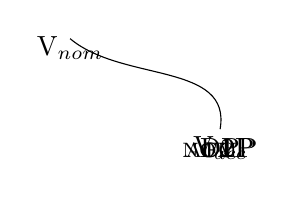
\begin{tikzpicture}[baseline,decoration={brace}]
\Tree [.\node(abovev){}; [.\node(V){V$_{nom}$}; ] 
[.\node(grow){}; ] ]
\begin{scope}[shift={(0.75in,-0.5in)}]
\Tree [.\node(bigtree){}; 
[.\node(Acc){\textsc{accP}};  [.\node(B){\textsc{f2}}; ]
[.\node(Nom){\textsc{nomP}};  [.\node(A){\textsc{f1}}; ]
[.\node(root){DP}; \edge[roof]; {} ] ] ] 
[ [.{...} ]
[.\node(V){V$_{acc}$}; ] ] ] ]
\end{scope}
\begin{scope}
\draw (grow.north) edge[out=320,in=80] (Nom.north);
\end{scope} 
\end{tikzpicture}

Next I discuss the situation in which the external case is more complex than the internal case, again accusative and nominative. A sentence from Old High German that illustrates this type of situation is given in \ref{ex:ohg-nom-acc-prev}, again repeated from earlier chapters.

\exg. Thíz ist then sie zéllent\\
\ac{dem}.\ac{sg}.\ac{n}.\ac{nom} be.\ac{pres}.3\ac{sg}\scsub{[nom]} \ac{rp}.\ac{sg}.\ac{m}.\ac{acc} 3\ac{pl}.\ac{m}.\ac{nom} tell.\ac{pres}.3\ac{pl}\scsub{[acc]}\\
`this is the one whom they talk about' \flushfill{Old High German, \ac{otfrid} III 16:50}\label{ex:ohg-nom-acc-prev}

The structure that corresponds to this sentence is given in \ref{ex:bergsma-nom-acc}. The relative clause on the right contains a predicate that takes nominative case, which appears on the left edge of the relative clause. The predicate in the main clause takes accusative case. The feature that makes the nominative an accusative is remerged with the nominative relative pronoun from the relative clause. The predicate from the main clause in turn is merged with the accusative node.

\ex.\label{ex:bergsma-nom-acc}
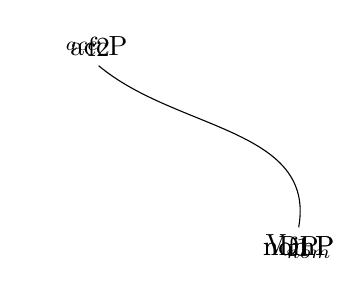
\begin{tikzpicture}[baseline,decoration={brace}]
\Tree [.\node(topnode){}; [.V$_{acc}$ ]
[.\node(Acc){\tsc{accP}}; [.\node(C){\tsc{f2}}; ] \edge[transparent];
[.\node(grow){}; ] ] ] ] ] ]
\begin{scope}[shift={(1.0in,-1.0in)}]
\Tree [.\node(free){\tsc{nomP}};
[.\node(Nom){\tsc{nomP}};  [.\node(A){\tsc{f1}}; ]
[.\node(root){DP}; \edge[roof]; {} ] ]
[ [.{...} ] 
[.\node(V){V$_{nom}$}; ] ] ]
\end{scope}
\draw (Acc.south) edge[out=320,in=80] (free.north);
\end{tikzpicture}

In sum, the account of \citet{bergsma2019} can be described in three derivational steps. 
In step 1, the relative clause predicate merges with the required case node. 
In step 2, the relative pronoun moves to the left edge of the clause. 
In step 3, the main clause predicate merges with the required case node. When the required case node is available, as in \ref{ex:bergsma-acc-nom}, this node is remerged with the main clause predicate. When the required case node is not available, as in \ref{ex:bergsma-nom-acc}, the highest case node is remerged with additional case features following the functional sequence until the required case node is merged, and then the main clause predicate is merged with the required case node. 

Variation between languages is formulated in terms of restrictions in step 3. A language without any restrictions is a language like Gothic: the relative pronoun always appears in the most complex case, no matter whether it is the internal or the external case. 

A language like Modern German has a restriction that is described as \textit{Keep spellout}: additional case features can only be merged to the relative pronoun if this does not change the spellout of the relative pronoun. As a result, when the internal case is more complex, a node within the relative pronoun can be remerged. However, when the internal case is less complex and additional case features need to be merged on top of the relative pronoun, this is prohibited. An exception is when it does not affect the spellout, which is how \citet{bergsma2019} accounts for syncretic forms being able to resolve a mismatch. 

A language like Polish has an additional restriction on top of the restriction that German has which is described as \textit{Only remerge highest node}: only the structurally highest node can be remerged with the main clause predicate. As a result, when the internal case is more complex, an embedded node cannot be remerged with the main clause predicate. Since Polish also has the restriction \textit{Keep spellout}, headless relatives with more complex external cases are also not grammatical, for the same reason as in Modern German.

\citet{bergsma2019} describes a fourth type of language, which is a language like Modern Greek, which is not described in this dissertation. This type of language only has the restriction \textit{Only remerge highest node} and not \textit{Keep spellout}. This means that headless relatives with a more complex internal case in Modern Greek are not grammatical, for the same reason as described for Polish above. When the external case is more complex, however, additional case features can be remerged with the relative pronoun. For Modern Greek this works in the same way as for languages like Gothic for the nominative/accusative cases. Exceptions are cases that involve a genitive. I give an example in \ref{ex:greek-nom-gen-prev}. We see the relative pronoun appearing in the case of the main clause (here nominative) and an additional resumptive pronoun in genitive appearing in the embedded clause, repeated from an earlier chapter. 

\exg. Me efχarístisan ópji tus íχa ðósi leftá.\\
 \ac{cl}.1\ac{sg}.\ac{acc} thank.\ac{pst}.3\ac{pl}\scsub{[nom]} \ac{rp}.\ac{pl}.\ac{m}.\ac{nom} \ac{cl}.3\ac{pl}.\ac{gen} have.\ac{pst}.1\ac{sg} give.\ac{ptcp}\scsub{[gen]} money\\
 `Whoever I had given money to, thanked me.'\flushfill{Modern Greek, adapted from \pgcitealt{daskalaki2011}{80}}\label{ex:greek-nom-gen-prev}

In a derivation similar to the ones discussed so far, this would mean that the relative pronoun first appears in the genitive case. Then when the main clause predicate requires a less complex case, part of the relative pronoun moves away to a place lower in the structure and spells out as a resumptive. This leaves a relative pronoun of which the highest node can be remerged. The movement of the resumptive pronoun is atypical, but the restrictions \textit{Keep spellout} and \textit{Only remerge highest node} fit the described pattern well.

This account and the one in this dissertation have in common how they model the case hierarchy: cases are represented by different nodes in the syntax and less complex cases are syntactically embedded in more complex cases. What differs is how the two accounts model the differences between languages. This starts with the assumptions about the underlying syntactic structure of the headless relative. The account in \citealt{bergsma2019} assumes that there is only a single element involved in case competition, which is the relative pronoun. Differences between languages follow from restrictions on whether the spellout of the relative pronoun can be changed and whether embedded features can be remerged. Unlike what is proposed in this dissertation, in which differences between languages follows from the internal structure of relative pronouns and light heads, these differences do not follow independently from properties of the language. There is no evidence from the morphology or from other constructions in a language that tells us whether the language has these restrictions, making them purely stipulative at this point. The account could be made stronger if there is evidence not from headless relatives that supports the need for the restrictions.


\section{Summary}

In this chapter I discussed three different proposals that account for different language types in headless relatives.
To account for the case facts, all of them refer in some way to a case hierarchy.
The accounts differ in how they model the variation between the languages. Of course there are differences in the mechanics of the proposals, but more importantly, there are differences in the empirical scope they have and the predictions they make.
What stands out is that all accounts except for the one in this dissertation include the Modern Greek pattern. Future research should point out how Modern Greek fits in the typology best and how the account set up in this dissertation can also account for this pattern.